\RequirePackage{luatex85}

\documentclass[tikz, border=10pt]{standalone}
\usepackage[compat=1.1.0]{tikz-feynman}


\begin{document}



% \feynmandiagram [horizontal=a to b] {
%   i1 [particle=\(e^{-}\)] -- [fermion] a -- [fermion] i2 [particle=\(e^{+}\)],
%   a -- [photon, edge label=\(Z^0\)] b,
%   f1 [particle=\(\bar{b}\)] -- [fermion] b -- [fermion] f2 [particle=\(b\)],
% };



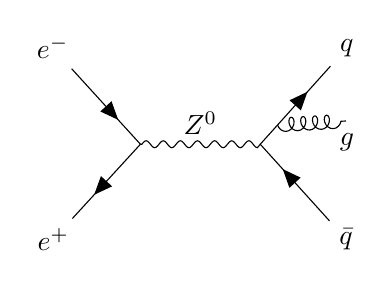
\begin{tikzpicture}
  \begin{feynman}
    \diagram [horizontal=a to b] {
      i1 [particle=\(e^+\)]
        -- [anti fermion] a
        -- [anti fermion] i2[particle=\(e^-\)],
      a -- [photon, edge label=\(Z^0\)] b,
      f1 [particle=\(q\)]
        -- [anti fermion] b
        -- [anti fermion] f2 [particle=\(\bar{q}\)]],
    };

    \vertex [above=of f2] (r);
    \draw [gluon] ($(f1)!0.8!(b)$) -- (r) node[below=of f1, yshift=0.3cm] {$g$};
    % \node[draw] below (r) {g};
  \end{feynman}
\end{tikzpicture}

\end{document}